%%%%%%%%%%%%%%%%%%%%%%%%%%%%%%%%%%%%%%%%%
% Cleese Assignment (For Students)
% LaTeX Template
% Version 2.0 (27/5/2018)
%
% This template originates from:
% http://www.LaTeXTemplates.com
%
% Author:
% Vel (vel@LaTeXTemplates.com)
%
% License:
% CC BY-NC-SA 3.0 (http://creativecommons.org/licenses/by-nc-sa/3.0/)
% 
%%%%%%%%%%%%%%%%%%%%%%%%%%%%%%%%%%%%%%%%%

%----------------------------------------------------------------------------------------
%	PACKAGES AND OTHER DOCUMENT CONFIGURATIONS
%----------------------------------------------------------------------------------------

\documentclass[10pt]{article}
%%%%%%%%%%%%%%%%%%%%%%%%%%%%%%%%%%%%%%%%%
% Cleese Assignment
% Structure Specification File
% Version 1.0 (27/5/2018)
%
% This template originates from:
% http://www.LaTeXTemplates.com
%
% Author:
% Vel (vel@LaTeXTemplates.com)
%
% License:
% CC BY-NC-SA 3.0 (http://creativecommons.org/licenses/by-nc-sa/3.0/)
% 
%%%%%%%%%%%%%%%%%%%%%%%%%%%%%%%%%%%%%%%%%

%----------------------------------------------------------------------------------------
%	PACKAGES AND OTHER DOCUMENT CONFIGURATIONS
%----------------------------------------------------------------------------------------

\usepackage{lastpage} % Required to determine the last page number for the footer


\usepackage{graphicx} % Required to insert images

\setlength\parindent{0pt} % Removes all indentation from paragraphs

\usepackage[svgnames]{xcolor} % Enabling colors by their 'svgnames'
\usepackage[most]{tcolorbox} % Required for boxes that split across pages

\usepackage{booktabs} % Required for better horizontal rules in tables

\usepackage{listings} % Required for insertion of code

\usepackage{etoolbox} % Required for if statements

\usepackage{multido} % required for dotted lines

% \usepackage{arydshln} % Required for dotted lines
% \setlength{\dashlinedash}{0.2pt}
% \setlength{\dashlinegap}{4.5pt}
% \setlength{\arrayrulewidth}{0.2pt}


\usepackage[french]{babel} % English language hyphenation

%----------------------------------------------------------------------------------------
%	MARGINS
%----------------------------------------------------------------------------------------

\usepackage{geometry} % Required for adjusting page dimensions and margins

\geometry{
	paper=a4paper, % Change to letterpaper for US letter
	top=2.5cm, % Top margin
	bottom=2cm, % Bottom margin
	left= 1.5cm, % Left margin
	right=1.5cm, % Right margin
	headheight=14pt, % Header height
	footskip=1.4cm, % Space from the bottom margin to the baseline of the footer
	headsep=1.2cm, % Space from the top margin to the baseline of the header
	%showframe, % Uncomment to show how the type block is set on the page
}


\usepackage{hyperref}
\hypersetup{%
  colorlinks=false,% hyperlinks will be black
  linkbordercolor=red,% hyperlink borders will be red
  pdfborderstyle={/S/U/W 1}% border style will be underline of width 1pt
}

\usepackage{awesomebox}
%----------------------------------------------------------------------------------------
%	FONT
%----------------------------------------------------------------------------------------
\usepackage{fontspec}
\usepackage{unicode-math}
\usepackage[utf8]{inputenc} % Required for inputting international characters
\usepackage[T1]{fontenc} % Output font encoding for international characters

% \usepackage[sfdefault,light]{roboto} % Use the Roboto font
\setmainfont[Ligatures=TeX]{Caladea}
%----------------------------------------------------------------------------------------
%	HEADERS AND FOOTERS
%----------------------------------------------------------------------------------------

\usepackage{fancyhdr} % Required for customising headers and footers

\pagestyle{fancy} % Enable custom headers and footers

\lhead{\small\assignmentClass\ifdef{\assignmentClassInstructor}{\ (\assignmentClassInstructor):}{}\ \assignmentTitle} % Left header; output the instructor in brackets if one was set
\chead{} % Centre header
\rhead{\small\ifdef{\assignmentAuthorName}{\assignmentAuthorName}{\ifdef{\assignmentDueDate}{Due\ \assignmentDueDate}{}}} % Right header; output the author name if one was set, otherwise the due date if that was set

\lfoot{} % Left footer
\cfoot{\small Page\ \thepage\ sur\ \pageref{LastPage}} % Centre footer
\rfoot{} % Right footer

\renewcommand\headrulewidth{0.5pt} % Thickness of the header rule


\fancypagestyle{plain}{
	\lhead{} % Left header; output the instructor in brackets if one was set
	\chead{} % Centre header
	\rhead{}

  \renewcommand{\headrulewidth}{0pt}%
  \fancyfoot[C]{\small Page\ \thepage\ sur\ \pageref{LastPage}}%
}

%----------------------------------------------------------------------------------------
%	MODIFY SECTION STYLES
%----------------------------------------------------------------------------------------

\usepackage{titlesec} % Required for modifying sections

%------------------------------------------------
% Section

\titleformat
{\section} % Section type being modified
[runin] % Shape type, can be: hang, block, display, runin, leftmargin, rightmargin, drop, wrap, frame
{\large} % Format of the whole section
{
\textbf{\assignmentQuestionName~\thesection :}	
} % Format of the section label
{6pt} % Space between the title and label
{} % Code before the label

\titlespacing{\section}
{-10pt}
{0.3\baselineskip}
{0.3\baselineskip} % Spacing around section titles, the order is: left, before and after

%------------------------------------------------
% Subsection

\titleformat
{\subsection} % Section type being modified
[block] % Shape type, can be: hang, block, display, runin, leftmargin, rightmargin, drop, wrap, frame
{\itshape \large} % Format of the whole section
{(\alph{subsection})} % Format of the section label
{4pt} % Space between the title and label
{} % Code before the label

\titlespacing{\subsection}
{0pt}
{0.3\baselineskip}
{0.3\baselineskip} % Spacing around section titles, the order is: left, before and after

\renewcommand\thesubsection{(\alph{subsection})}

%----------------------------------------------------------------------------------------
%	CUSTOM QUESTION COMMANDS/ENVIRONMENTS
%----------------------------------------------------------------------------------------

% Environment to be used for each question in the assignment
\newenvironment{question}{
	\vspace{0.2\baselineskip} % Whitespace before the question
	\section{} % Blank section title (e.g. just Question 2)
	\lfoot{La \small\itshape\assignmentQuestionName~\thesection~continue sur la page d'après\ldots} % Set the left footer to state the question continues on the next page, this is reset to nothing if it doesn't (below)
}
{
	\lfoot{} % Reset the left footer to nothing if the current question does not continue on the next page
}

%------------------------------------------------

% Environment for subquestions, takes 1 argument - the name of the section
\newenvironment{subquestion}[1]{
	\subsection{#1}
}{
}

%------------------------------------------------

% Command to print a question sentence
\newcommand{\questiontext}[1]{
	\large #1
	\vspace{0.2\baselineskip} % Whitespace afterwards
}

%------------------------------------------------

% Command to print a box that breaks across pages with the question answer
\newcommand{\answer}[1]{
	\begin{tcolorbox}[breakable, enhanced]
		#1
	\end{tcolorbox}
}

%------------------------------------------------

% Command to print a box that breaks across pages with the space for a student to answer
\newcommand{\answerbox}[1]{
	\begin{tcolorbox}[breakable, enhanced]
		% \vphantom{L}
		% \vspace{\numexpr #1-1\relax\baselineskip} % \vphantom{L} to provide a typesetting strut with a height for the line, \numexpr to subtract user input by 1 to make it 0-based as this command is
		\vspace{15pt}
		\multido{}{#1}{\noindent\makebox[\linewidth]{\dotfill}
		\endgraf\vspace{12pt}}% ... dotted lines ...
		\vspace{-13pt}
	\end{tcolorbox}
}


\newtcolorbox{mybox}[1][]{
    colbacktitle=blue!10!white,
    colback=red!10!white,
    coltitle=blue!70!black,
    adjusted title={#1},
    fonttitle=\bfseries,
    % attach title to upper={\ --- \ }
    }

%------------------------------------------------

% Command to print an assignment section title to split an assignment into major parts
\newcommand{\assignmentSection}[1]{
	{
		\centering % Centre the section title
		\vspace{1\baselineskip} % Whitespace before the entire section title
		
		\rule{0.8\textwidth}{0.5pt} % Horizontal rule
		
		\vspace{0.75\baselineskip} % Whitespace before the section title
		{\LARGE \MakeUppercase{#1}} % Section title, forced to be uppercase
		
		\rule{0.8\textwidth}{0.5pt} % Horizontal rule
		
		\vspace{\baselineskip} % Whitespace after the entire section title
	}
}


%	TITLE SECTION
%----------------------------------------------------------------------------------------

% \newcommand{\authorstyle}[1]{{\large\usefont{OT1}{phv}{b}{n}#1}} % Authors style (Helvetica)

% \newcommand{\institution}[1]{{\footnotesize\usefont{OT1}{phv}{m}{sl}#1}} % Institutions style (Helvetica)

\usepackage{titling} % Allows custom title configuration

\newcommand{\HorRule}{\rule{\linewidth}{1pt}} % Defines the gold horizontal rule around the title

\pretitle{
	\centering
	\vspace{-120pt} % Move the entire title section up
	\HorRule\vspace{10pt} % Horizontal rule before the title
	% \textbf
	\bfseries
	\fontsize{32}{36}
	\usefont{T1}{phv}{b}{n}
	\selectfont % Helvetica
	\color{DarkRed} % Text colour for the title and author(s)
}

\posttitle{\par\vskip 15pt} % Whitespace under the title

\preauthor{} % Anything that will appear before \author is printed

\postauthor{ % Anything that will appear after \author is printed
	% \vspace{10pt} % Space before the rule
	\par\HorRule % Horizontal rule after the title
	\vspace{-40pt} % Space after the title section
}

\usepackage{blindtext, subfig}
\usepackage{dblfloatfix} % fix for bottom-placement of figure % Include the file specifying the document structure and custom commands
% \usepackage{activite}
%----------------------------------------------------------------------------------------
%	ASSIGNMENT INFORMATION
%----------------------------------------------------------------------------------------

% Required
\newcommand{\assignmentQuestionName}{Question} % The word to be used as a prefix to question numbers; example alternatives: Problem, Exercise
\newcommand{\assignmentClass}{Physique Chimie} % Course/class
\newcommand{\assignmentTitle}{Activité n°1} % Assignment title or name
\newcommand{\assignmentAuthorName}{Chapitre 3} %

%----------------------------------------------------------------------------------------
%	VARIABLES
%----------------------------------------------------------------------------------------

\newcommand{\titreActivite}{Activité 1: Le Volume} % titre de l'activité
\newcommand{\objectif}{ 	
	
	\begin{itemize}
		\item Notion de volume.
		\item Savoir mesurer un volume.
	\end{itemize}
}
\newcommand{\contexte}{
	Abdel et Sohane ont décidé de préparer des pancakes avec leur mère
	pour le goûter. En ouvrant le livre de recette, nous obtenons la liste des
	ingrédients suivante :
	\begin{itemize}
		\item  2 Œufs.
		\item  15 g de sucre en poudre.
		\item  10 mL d’huile d’olive.
		\item  300 g de farine.
		\item  1 sachet de levure.
		\item  400 mL de lait.
	\end{itemize}
	Ils savent comment obtenir précisément 15 g de sucre ou 300 g de farine mais 
	sont bien embétés pour obtenir 10 mL d’huile d’olive ou 400 mL de lait.
}
\newcommand{\resumeContexte}{
	Saura-tu aider Abdel et Sohane à faire des pancakes?
	}


%----------------------------------------------------------------------------------------

\begin{document}
%----------------------------------------------------------------------------------------
%	TITLE PAGE
%----------------------------------------------------------------------------------------
\date{}
\title{\titreActivite}
\maketitle % Print the title page

%----------------------------------------------------------------------------------------
%	QUESTION 1
%----------------------------------------------------------------------------------------

\begin{minipage}[c]{0.5\textwidth}
	\underline{\textbf{Objectif}} :  \vspace{2pt}
	\objectif

	\vspace{4pt}


    \underline{\textbf{Contexte}} :  \textit{\contexte}
\end{minipage} 
\hspace{10pt}
\begin{minipage}[c]{0.45\textwidth}
	\begin{center}
		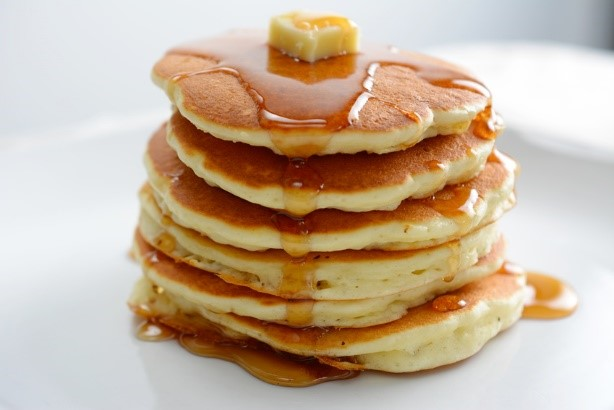
\includegraphics[width=0.8\columnwidth]{assets/img_-001.png} % Example image
	\end{center}

	\textbf{\resumeContexte}
\end{minipage}

% \vspace{-12pt}
%% ----------------------------------

\assignmentSection{Votre mission travail}

%----------------------------------------------------------------------------------------
%	QUESTION 1
%----------------------------------------------------------------------------------------

\begin{question}
	\questiontext{
		La mère de nos deux cuisiniers essaye de résoudre leur problème en leur donnant l’ustensile ci-dessous,
		comment celui-ci s’appelle-t-il ? A quoi sert-t-il ?
	}
\end{question}

\hspace{30pt}
\begin{minipage}[c]{0.25\textwidth}
    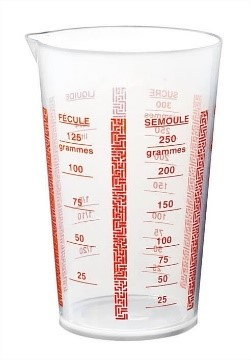
\includegraphics[width=0.5\textwidth]{assets/img_-002.png}
\end{minipage} 
\hspace{-30pt}
\begin{minipage}[c]{0.75\textwidth}
\answerbox{2}
\end{minipage}


\begin{question}
	\questiontext{
		En chimie, nous utilisons du matériel adapté à la mesure du volume.
		Connais-tu le noms de la verrerie suivante?
	}
\end{question}

\makebox(0,20){}

\begin{minipage}[c]{0.3\textwidth}
	\begin{minipage}[c]{0.45\textwidth}
		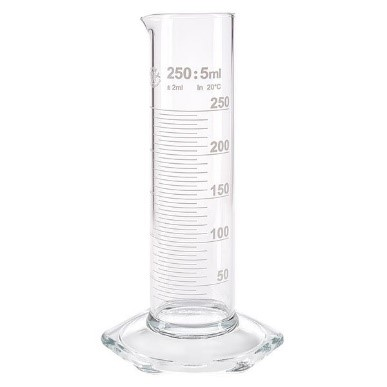
\includegraphics[width=\textwidth]{assets/img_-003.png}
	\end{minipage} 
	\begin{minipage}[c]{0.45\textwidth}
		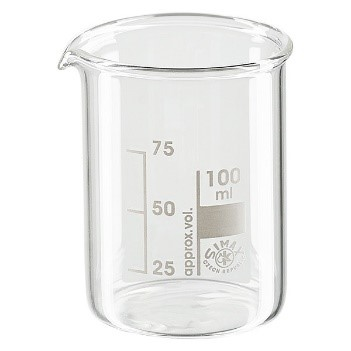
\includegraphics[width=\textwidth]{assets/img_-004.png}
	\end{minipage} 
\end{minipage} \hspace{10pt}
\begin{minipage}[c]{0.65\textwidth}
	\answerbox{3}
\end{minipage}

\newpage

\begin{question}
	\questiontext{
		A partir du tableau de conversion ci-dessous, convertir les volumes donnés dans les unités demandées
\begin{center}
	\begin{itemize}
		\item Une bouteille d’eau : 1L = ............. mL
		\item Une canette de soda de 33 cL = ............. mL = ............. L
		\item Une bassine d’eau : 3500 mL = .............. L
		\item Une baignoire remplie d’eau : 120 L = ........... mL
	\end{itemize}   
\end{center} 
 }
\end{question}

\begin{center}
	\begin{tabular}{ |c|c|c|c|c|c|c|  }
		\hline
		\multicolumn{7}{|c|}{\makebox(0,20){} Tableau de conversion} \\\hline
		\makebox(0,20){} \hspace{10pt} Kilolitre \hspace{10pt} &\hspace{10pt}  Hectolitre \hspace{10pt} &\hspace{10pt}  Décalitre \hspace{10pt} &\hspace{10pt}  litre \hspace{10pt} & \hspace{10pt} Décilitre\hspace{10pt}  & \hspace{10pt} Centilitre \hspace{10pt} & \hspace{10pt} Millilitre\hspace{10pt}  \\\hline% \makebox(0,15){}
		\makebox(0,20){} &  &  &  &  &  &  \\\hline% 
		\makebox(0,20){} &  &  &  &  &  &  \\\hline% 
		\makebox(0,20){} &  &  &  &  &  &  \\\hline% 
		\makebox(0,20){} &  &  &  &  &  &  \\\hline% 
	\end{tabular}
\end{center}

\begin{question}
	\questiontext{
		Indiquer la valeur du volume mesuré pour les éprouvettes a, b, c et d.
	\vspace{10pt}

	\begin{minipage}[c]{0.45\textwidth}
		\begin{center}
			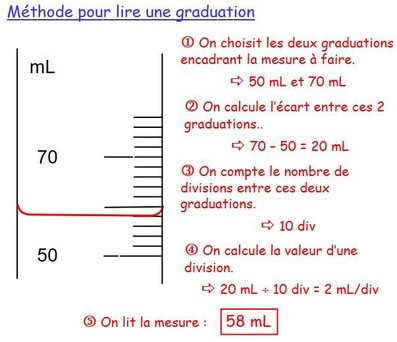
\includegraphics[width=\textwidth]{assets/img_-011.png}
		\end{center}		
	\end{minipage} \hspace{10pt}
	\begin{minipage}[c]{0.5\textwidth}
		Pour lire précisément la graduation concernant la valeur
		de notre volume, il faut :
		Dans une ...................................................., il faut lire la
		graduation qui correspond au bas du ménisque. Le
		ménisque est le creux que forme la surface libre d'un
		liquide.
		\begin{center}
			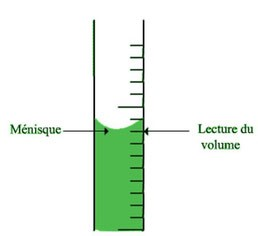
\includegraphics[width=0.5\textwidth]{assets/img_-013.png}
		\end{center}	
	\end{minipage}
	\begin{center}
		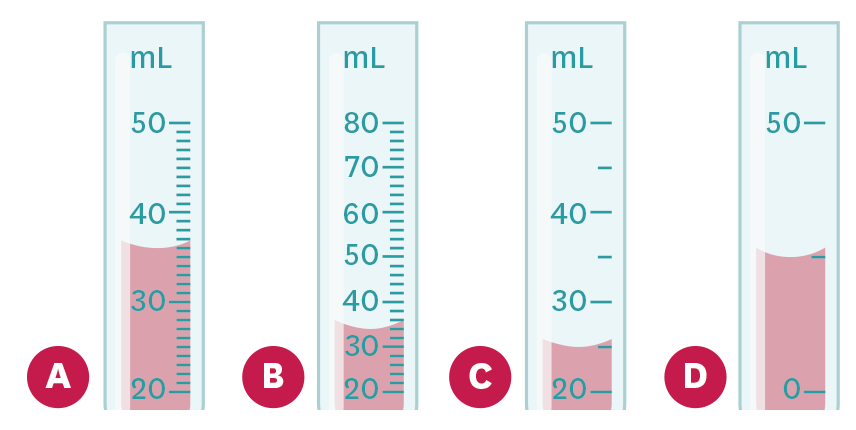
\includegraphics[width=0.5\textwidth]{assets/img_-012.png}
	\end{center}

}
\end{question}
\answerbox{2}

\begin{question}
	\questiontext{
	Mesurer 15 mL d'eau dans une éprouvette puis appeler 
	l'enseignant.e pour vérification.
}
\end{question}

\end{document}
